\documentclass[oneside]{unilasalle}

\usepackage[T1]{fontenc}
\usepackage{float}
\usepackage[latin1]{inputenc}
\usepackage{latexsym}
\usepackage{psfrag}
\usepackage{amssymb}
\usepackage{subfig}

\usepackage{url}
\usepackage{listings}
\lstset{
  basicstyle  = \footnotesize\ttfamily,
  stringstyle = \ttfamily,
  numberstyle = \scriptsize\ttfamily
}




%%%%%%

%
% Informacoes gerais => tirado do exemplo-tc.tex do Vinicius Mingot
%
\title{Monitoramento de Recursos em Ambientes de Grade}

\author{Lemos}{Daniel da Trindade}

\advisor[Profa.~DSc.]{Mangan}{Patr�cia Kayser Vargas}

% a data deve ser a da defesa; se n�o especificada, s�o gerados
% m�s e ano correntes
%\date{novembro}{2006}

% o nome do curso pode ser redefinido
\course{Ci�ncia da Computa��o}

%
% palavras-chave
% iniciar todas com letras min�sculas, exceto no caso de abreviaturas
%
\keyword{computa��o em grade}
\keyword{monitoramento}
\keyword{{\it Web services}}


%%%%%%

\begin{document}
%	%------------------------------------------------------------------------------------------------
% \simb[entrada na lista de s�mbolos]{s�mbolo}:
%   Escreve o simbolo no texto e uma entrada na Lista de S�mbolos.
%   Se o par�metro opcional e omitido, usa-se o par�metro obrigat�rio.
%------------------------------------------------------------------------------------------------
\newcommand{\simb}[2][]{%
  \ifthenelse{\equal{#1}{}}
    {\addcontentsline{los}{simbolo}{\ensuremath{#2}}}
    {\addcontentsline{los}{simbolo}{#1}}
  \ensuremath{#2}
}

\makeatletter
%------------------------------------------------------------------------------------------------
% \listadesimbolos: comando que imprime a lista de simbolos
%------------------------------------------------------------------------------------------------
\newcommand{\listadesimbolos}{
  \pretextualchapter{Lista de S�mbolos}
  {\setlength{\parindent}{0cm}
   \@starttoc{los}}}

\newcommand\listabbrname{Lista de S\'imbolos e Abreviaturas}
\newcommand\listofabbreviations{%
    \chapter*{\listabbrname
      \@mkboth{\MakeUppercase\listabbrname\space\draftdate}%
              {\MakeUppercase\listabbrname\space\draftdate}}%
     % \addcontentsline{toc}{chapter}{\MakeUppercase\listabbrname}%
    \@starttoc{lob}%
    }
\newcommand\abbrev[2]{%
                                        \def\({$}%
                                        \def\){$}%
      \addcontentsline{lob}{section}{%
                                                                \rm%
                        \protect\parbox[t]{.2\textwidth}{\bf #1}%
                   \hspace{0.025\textwidth}%
                   \protect\parbox[t]{.6\textwidth}{#2}%
        \vspace{2mm}\hspace{.1\textwidth}}%
      }

%------------------------------------------------------------------------------------------------
% como a entrada ser� impressa
\newcommand\l@simbolo[2]{\par #1, p.\thinspace#2}
		% pkvm %
	
%
% inicio do documento
%

% capa
\maketoppage

% folha de rosto
%\maketitle

\thetitlepage
\makeappage

% dedicatoria
%\clearpage
%\begin{flushright}
%\mbox{}\vfill
%{\sffamily\itshape
%``If I have seen farther than others,\\
%it is because I stood on the shoulders of giants.''\\}
%--- \textsc{Sir~Isaac Newton}
%\end{flushright}

% agradecimentos
\chapter*{Agradecimentos}

\begin{abstract}
O processamento distribuído através das Grades computacionais, conta com uma grande infra-estrutura de redes. Esta infra-estrutura pode ser empregada em troca de programas, dados e serviços. Para gerenciar essa diversidade de aplicações destacam-se os Sistemas Gerenciadores de Recursos (RMS), esses sistemas tem por função gerenciar de forma cooperativa e transparente os recursos geograficamente distribuídos considerando-os como pertencentes de um único computador. Neste contexto apresenta-se o protótipo AppMan baseado no modelo GRAND ({\bf G}rand {\bf R}obust {\bf A}pplicatio{\bf n} {\bf D}eployment). Esse protótipo não implementa por completo o que sugere o modelo, dentre das características não implementadas, cita-se a integração com diferentes RMS. Através de estudos encontrou-se a Implementação DRMMA ({\bf D}istribuited {\bf R}esource {\bf M}anagement {\bf A}pplication {\bf A}PI) que visa integrar diferentes RMS. Este trabalho demonstra a viabilidade da integração do protótipo AppMan com o RMS PBS através da DRMAA. Os testes comprovaram que, apesar da necessidade de inúmeras melhorias no protótipo, a integração é possível com pouco intrusão no código atual. A versão da DRMAA usada foi o pacote na linguagem Java que é a mesma linguagem do protótipo.
\end{abstract}

\begin{englishabstract}{}{Grid Computing, Resource Management}
The processing distributed through Grid Computing, has a large infrastructure networks. This infrastructure can be used in exchange of programs, data and services. To manage this diversity of applications are the Resource Management System (RMS), these systems is to manage in a cooperative and transparent the resource geographically distributed considering them as belonging to a single computer. In this context is theconsidering them as belonging to a single computer. In this context is the prototype model based on AppMan GRAND ({\bf G}rand {\bf R}obust {\bf A}pplicatio{\bf n} {\bf D}eployment). This prototype not completely implemented, refers to the integration with different RMS. Through studies found himself the Implementation DRMAA ({\bf D}istribuited {\bf R}esource {\bf M}anagement {\bf A}pplication {\bf A}PI) which aims to integrate different RMS. This resource demonstrates the feasibility of integrating the prototype AppMan with the RMS PBS through DRMAA. Tests have shown that, despite the need for numerous improvements in the prototype, integration is possible with little intrusion in the current code. The DRMAA version of the package was used in the Java language that is the same language of the prototype.
\end{englishabstract}		% pkvm %
	%dtl%\begin{resumo}
%pkvm%
\begin{abstract}
Em um ambiente de computa��o em grade, ...  Assim, este trabalho busca um modelo de monitoramento de recursos de
hardware e software, que contemple as quest�es de escalabilidade e
heterogeneidade,para ambientes de grade. 
Um prot�tipo foi implementado ... . As avalia��es mostraram ....






%O Sistema Operacional atendido pelo prot�tipo � Windows. 
%Uma vez com o prot�tipo finalizado, foi utilizado como ambiente de teste o laborat�rio do Banrisul \abbrev{BANRISUL}{Banco %do %Estado do Rio Grande do Sul}.Os resultados da mo\-ni\-to\-ra\-��o ser�o disponibilizados no formato XML %\abbrev{XML}{\emph{eXtensible Markup Language}} para facilitar a integra��o com outras ferramentas.

%Posteriormente, deseja-se montar uma grade de teste envolvendo m�quinas do laborat�rio 24h do Unilasalle, da UFRJ %\abbrev{UFRJ}{Universidade Federal do Rio de Janeiro} e da UFLA\abbrev{UFLA}{Universidade Federal de Lavras} para teste do %sensor Linux. Os resultados da mo\-ni\-to\-ra\-��o ser�o 
%disponibilizados no formato XML \abbrev{XML}{\emph{eXtensible Markup Language}} para facilitar 
%a integra��o com outras ferramentas.
%dtl%\end{resumo}
%dtl%\begin{abstract}
\end{abstract}

% resumo na outra l�ngua
% como parametros devem ser passados o titulo e as palavras-chave
% na outra l�ngua, separadas por v�rgulas

%\selectlanguage{english}

\begin{englishabstract}{Resource Monitoring in Grid Environments}{Grid Computing, Monitoring, Web Services}
In a grid computing environment, ...
Thus, this work aims at proposing a hardware and software resource
monitoring model for grid environment, which deals with scalability
and heterogeneity issues.
A prototype was implemented ... The evaluation showed ...
\end{englishabstract}

%\selectlanguage{brazilian}

		% pkvm %
	
% sumario
\tableofcontents

% lista de abreviaturas e siglas
% o parametro deve ser a abreviatura mais longa

\begin{listofabbrv}{SPMD}
        \item[RMS]   \emph{Resource Management System}
        \item[GRAND] \emph{Grid Robust Application Deployment}
        \item[DRMAA] \emph{Distributed Resource Management Application}
        \item[API]   \emph{Application Program Interface}
        \item[ISAM]  Infra-estrutura de Suporte às Aplicações Móveis
        \item[EXEHDA]\emph{Execution Environment for Highly Distributed Applications}
        \item[LDAP]  \emph{Lightweight Directory Access Protocol}
        \item[UML]   \emph{Unified Modeling Language}
        \item[OGF]   \emph{Open Grid Forum}
        \item[GT]    \emph{Globus Toolkit}
        \item[PBS]   \emph{Portable Batch System}
        \item[MDS]   \emph{Metacomputing Directory Services}
        \item[GRAM]  \emph{Globus Resource Allocation Manager}
        \item[OGSA]  \emph{Open Grid Services Architecture}
        \item[WSRF]  \emph{Web Services Resource Framework}
        \item[AP]    \emph{Application Manager}
        \item[SM]    \emph{Submission Manager}
        \item[TM]    \emph{Task Manager}
\end{listofabbrv}

%\listofabbreviations

% lista de figuras
\listoffigures

% lista de tabelas
\listoftables

		% pkvm %

	\chapter{Introdu��o}
\label{cap:introducao}


Foster et al. \cite{fosterGridChapterBook98} define uma grade como um sistema que ...


O restante deste texto apresenta-se organizado do seguinte modo. Inicialmente, apresentam-se o Cap�tulo \ref{cap:Monitoramento_Grade} sobre Monitoramento em Grade, onde ser� abordado as principais ferramentas de monitoramento existentes hoje em grades computacionais. Depois ter� o Cap�tulo \ref{cap:Modelo} com o modelo, onde tratar� principalmente das premissas, dos dados monitorados e da modelagem e prot�tipo. Depois, o Cap�tulo \ref{cap:Dados_Experimentais} analisa os resultados obtidos com os experimentos efetuados. Finalmente ter� o cap�tulo \ref{cap:Conclusao} concluido este texto tamb�m abordando os trabalhos futuros.
 		% Inclus�o da Introdu��o
	\chapter{Monitoramento em Grade}
\label{cap:Monitoramento_Grade}

...


Segundo Jain \cite{jain91} um monitor � uma ferramenta utilizada para ...


As informa��es de monitoramento de hardware e software devem ser coletadas m�quina a m�quina, mas normalmente s�o
centralizadas nas redes locais ou {\it clusters}. 


\section{\label{sec_Trab_Relacionados}Trabalhos Relacionados}

 ...

\subsection{\label{subsec_Ganglia}Ganglia}

...

\subsection{\label{subsec_Condor_Hawkeye}Condor e Hawkeye}

...


\subsection{\label{sec_globus_WebMds}Globus e WebMDS}



\subsection{\label{subsec_Grads_NWS}GrADS e NWS}

...


\section{\label{sec_analise}An�lise}

...	% Inclus�o do Capitulo de Monitoramento
	\section{Modelo Proposto}
\label{cap:modelo proposto}


O protótipo AppMan é uma implementação simplificada do GRAND. Ele usa a ferramenta JavaCC para implementar o {\it parsing} e interpretação da GRID-ADL. A Figura 2 representa um possível cenário do AppMan sendo executado sobre um ambiente de grade.

O passo 1 da figura representa o usuário submetendo um arquivo de descrição na linguagem GRID-ADL. Esse arquivo é analisado e o grafo de aplicação é feito na memória. Um algoritmo é executado e os sub-DAGs do grafo de aplicação é obtido. O {\it Application Manager} (AM) é inicializado. Então o AM instância {\it Submission Managers} (SM) no passo 2 e distribui alguns subgrafos para os SMs. Os arquivos de entrada e os executáveis são obtidos através de um {\it web server} (passo 3). Na sua atual implementação, AppMan necessita que o usuário indique as máquinas onde os SMs irão ser executados. Com essa simplificação um novo SM é instanciado para cada aplicação em cada máquina especificada. Após a criação dos SMs, o AM determina sub-grafos para cada SM. Os SMs informam para o AM o progresso das tarefas. Cada SM, independentemente, verifica a lista das máquinas disponíveis e escolhe aleatoriamente um nó para executar a tarefa. Antes de iniciar a execução de uma tarefa, o AppMan transfere todos arquivos de entradas especificados na descrição GRID-ADL para um diretório temporário no nó remoto onde a tarefa será executada. O arquivo de transferência é executado automaticamente. Então, cada SM recupera a informação atualizada através do serviço de informação do EXEHDA sobre os nós avaliados. Cada SM escolhe onde irá executar estas tarefas aleatoriamente. Imediatamente um {\it Task Manameger} (TM) é instanciado criando a tarefa remota e monitorando até que a execução da tarefa termine (passo 4).

\begin{figure}[hbtp]
\center
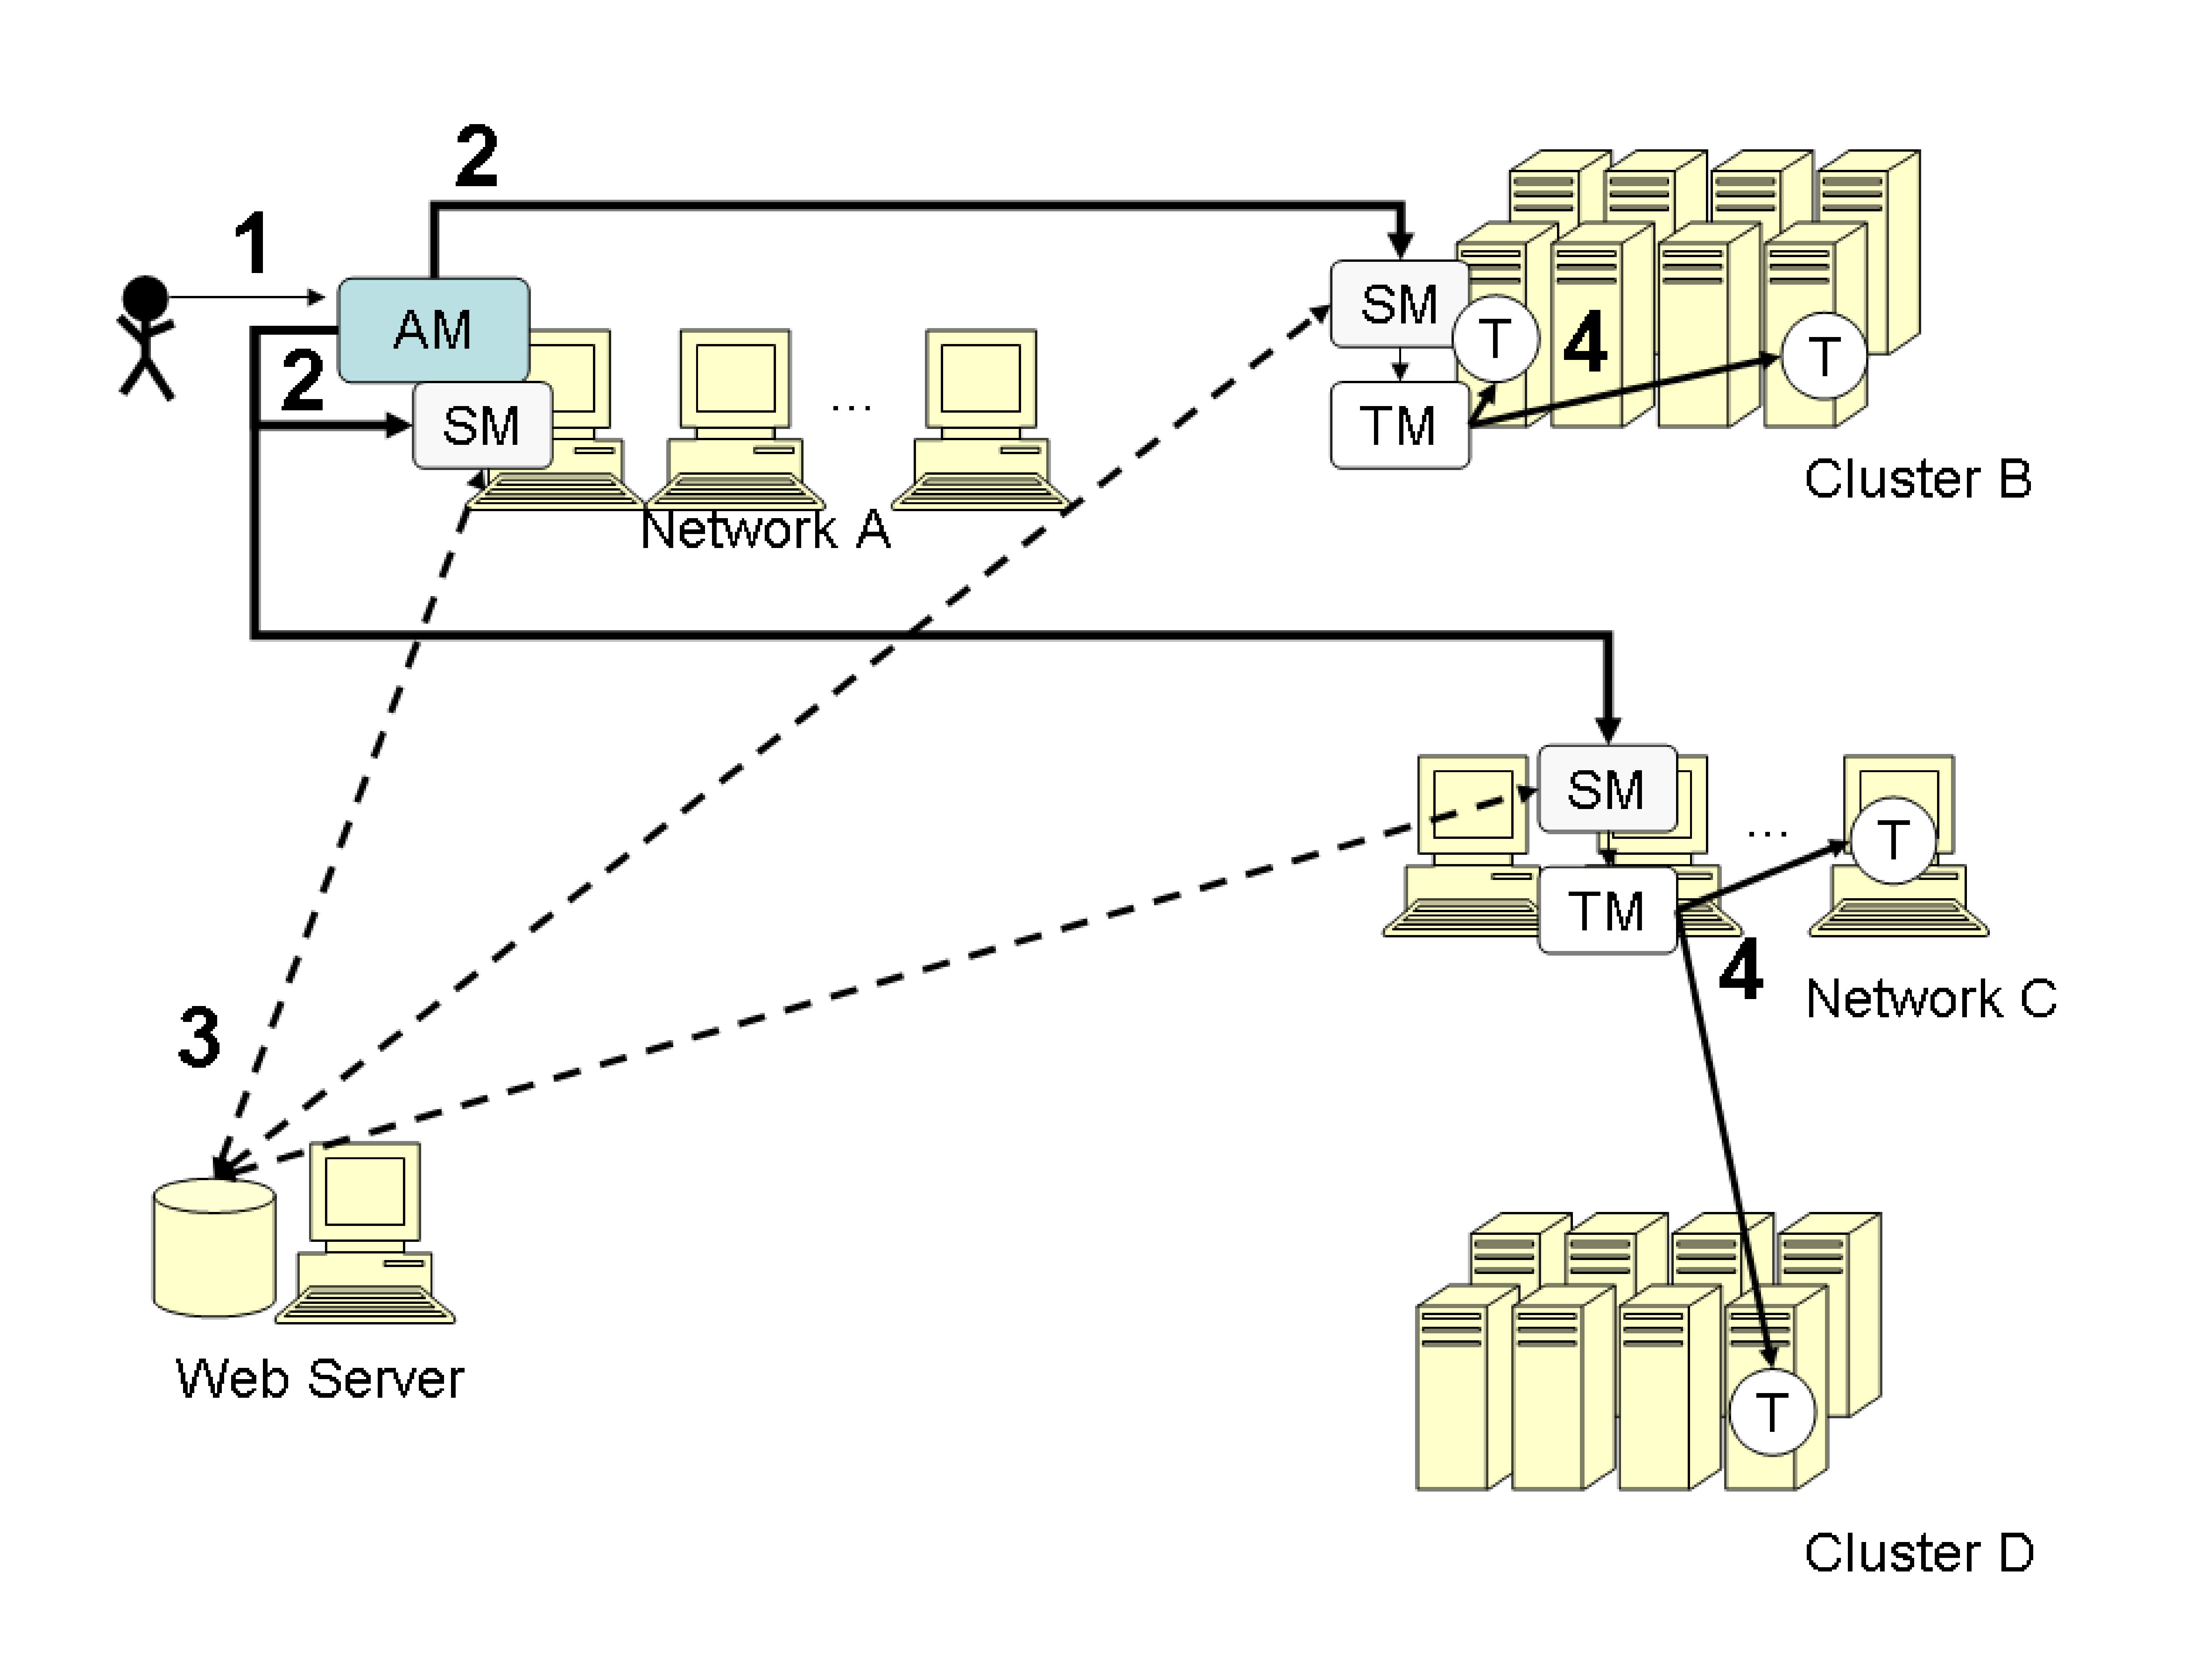
\includegraphics[scale=.1]{img/AppMan.eps}
\label{AppMan}
\caption{AppMan executando principais passos}
\end{figure}

Como sugere o modelo GRAND, o AppMan não possibilita o escalonamento através de outros RMSs. É necessário que o EXEHDA e o AppMan estejam presentes em todos nós da grade. Integrar o AppMan com outros RMS possibilitará uma maior escalabilidade da grade e também possibilitará uma aproximação do AppMan ao que sugere o modelo GRAND. Os nós principais de cada {\it cluster} que compõem a base possuem nós abaixo delas. O AppMan espera um serviço de compartilhamento de arquivo entre os nós e base. Isto é, mais uma característica que impossibilita o uso de nós da grade sem NFS, como existente na parceria LNCC/Petrópolis-RJ, pelo AppMan.

Uma especificação {\it Distributed Resource Management Application} \cite{Rajic2002} desenvolvida pelo OGF, tem por objetivo abstrair as diferenças dos RMS e fornecer uma API visando facilitar a integração de aplicações. O escopo da DRMAA é limitada a submissão, monitoramento e controle das tarefas além de retornar status de conclusão de uma tarefa. Inicialmente implementada na linguagem C, atualmente possui uma implementação na linguagem Java, apesar de oferecer suporte apenas para o {\it Sun Grid Engine} \cite{Templeton}.

Vários relatórios técnicos N1™ Grid Engine \cite{Templeton2006}, GridWay \cite{Herrera2007}, Condor \cite{Troeger2007} e PBS \cite{Ciesnik2007} existentes da implementação DRMAA, concluem positivamente. Além disso demonstraram uma pequena necessidade de inteferência no código dos RMSs citados.

Em um primeiro estudo da documentação do AppMan pode-se notar duas principais classes, {\it TaskManager} e {\it SubmissionManager}. A classe {\it SubmissionManager} implementa os métodos da {\it Interface SubmissionManagerRemote} a qual possui os métodos que recuperam informações das tarefas executadas remotamente e o metódo da geração do grafo da aplicação. A classe {\it TaskManager } implementa a interface {\it TaskManagerRemote} contendo os métodos tais como os que adicionam tarefas na lista de execução remota.  A Figura 3 mostra o diagrama simplificado de classes do AppMan. Nesta figura estão circuladas as duas classes que foram identificadas até o momento como sendo necessário algum tipo de adaptação para a implementação do presente trabalho.

\begin{figure}[h]
\center
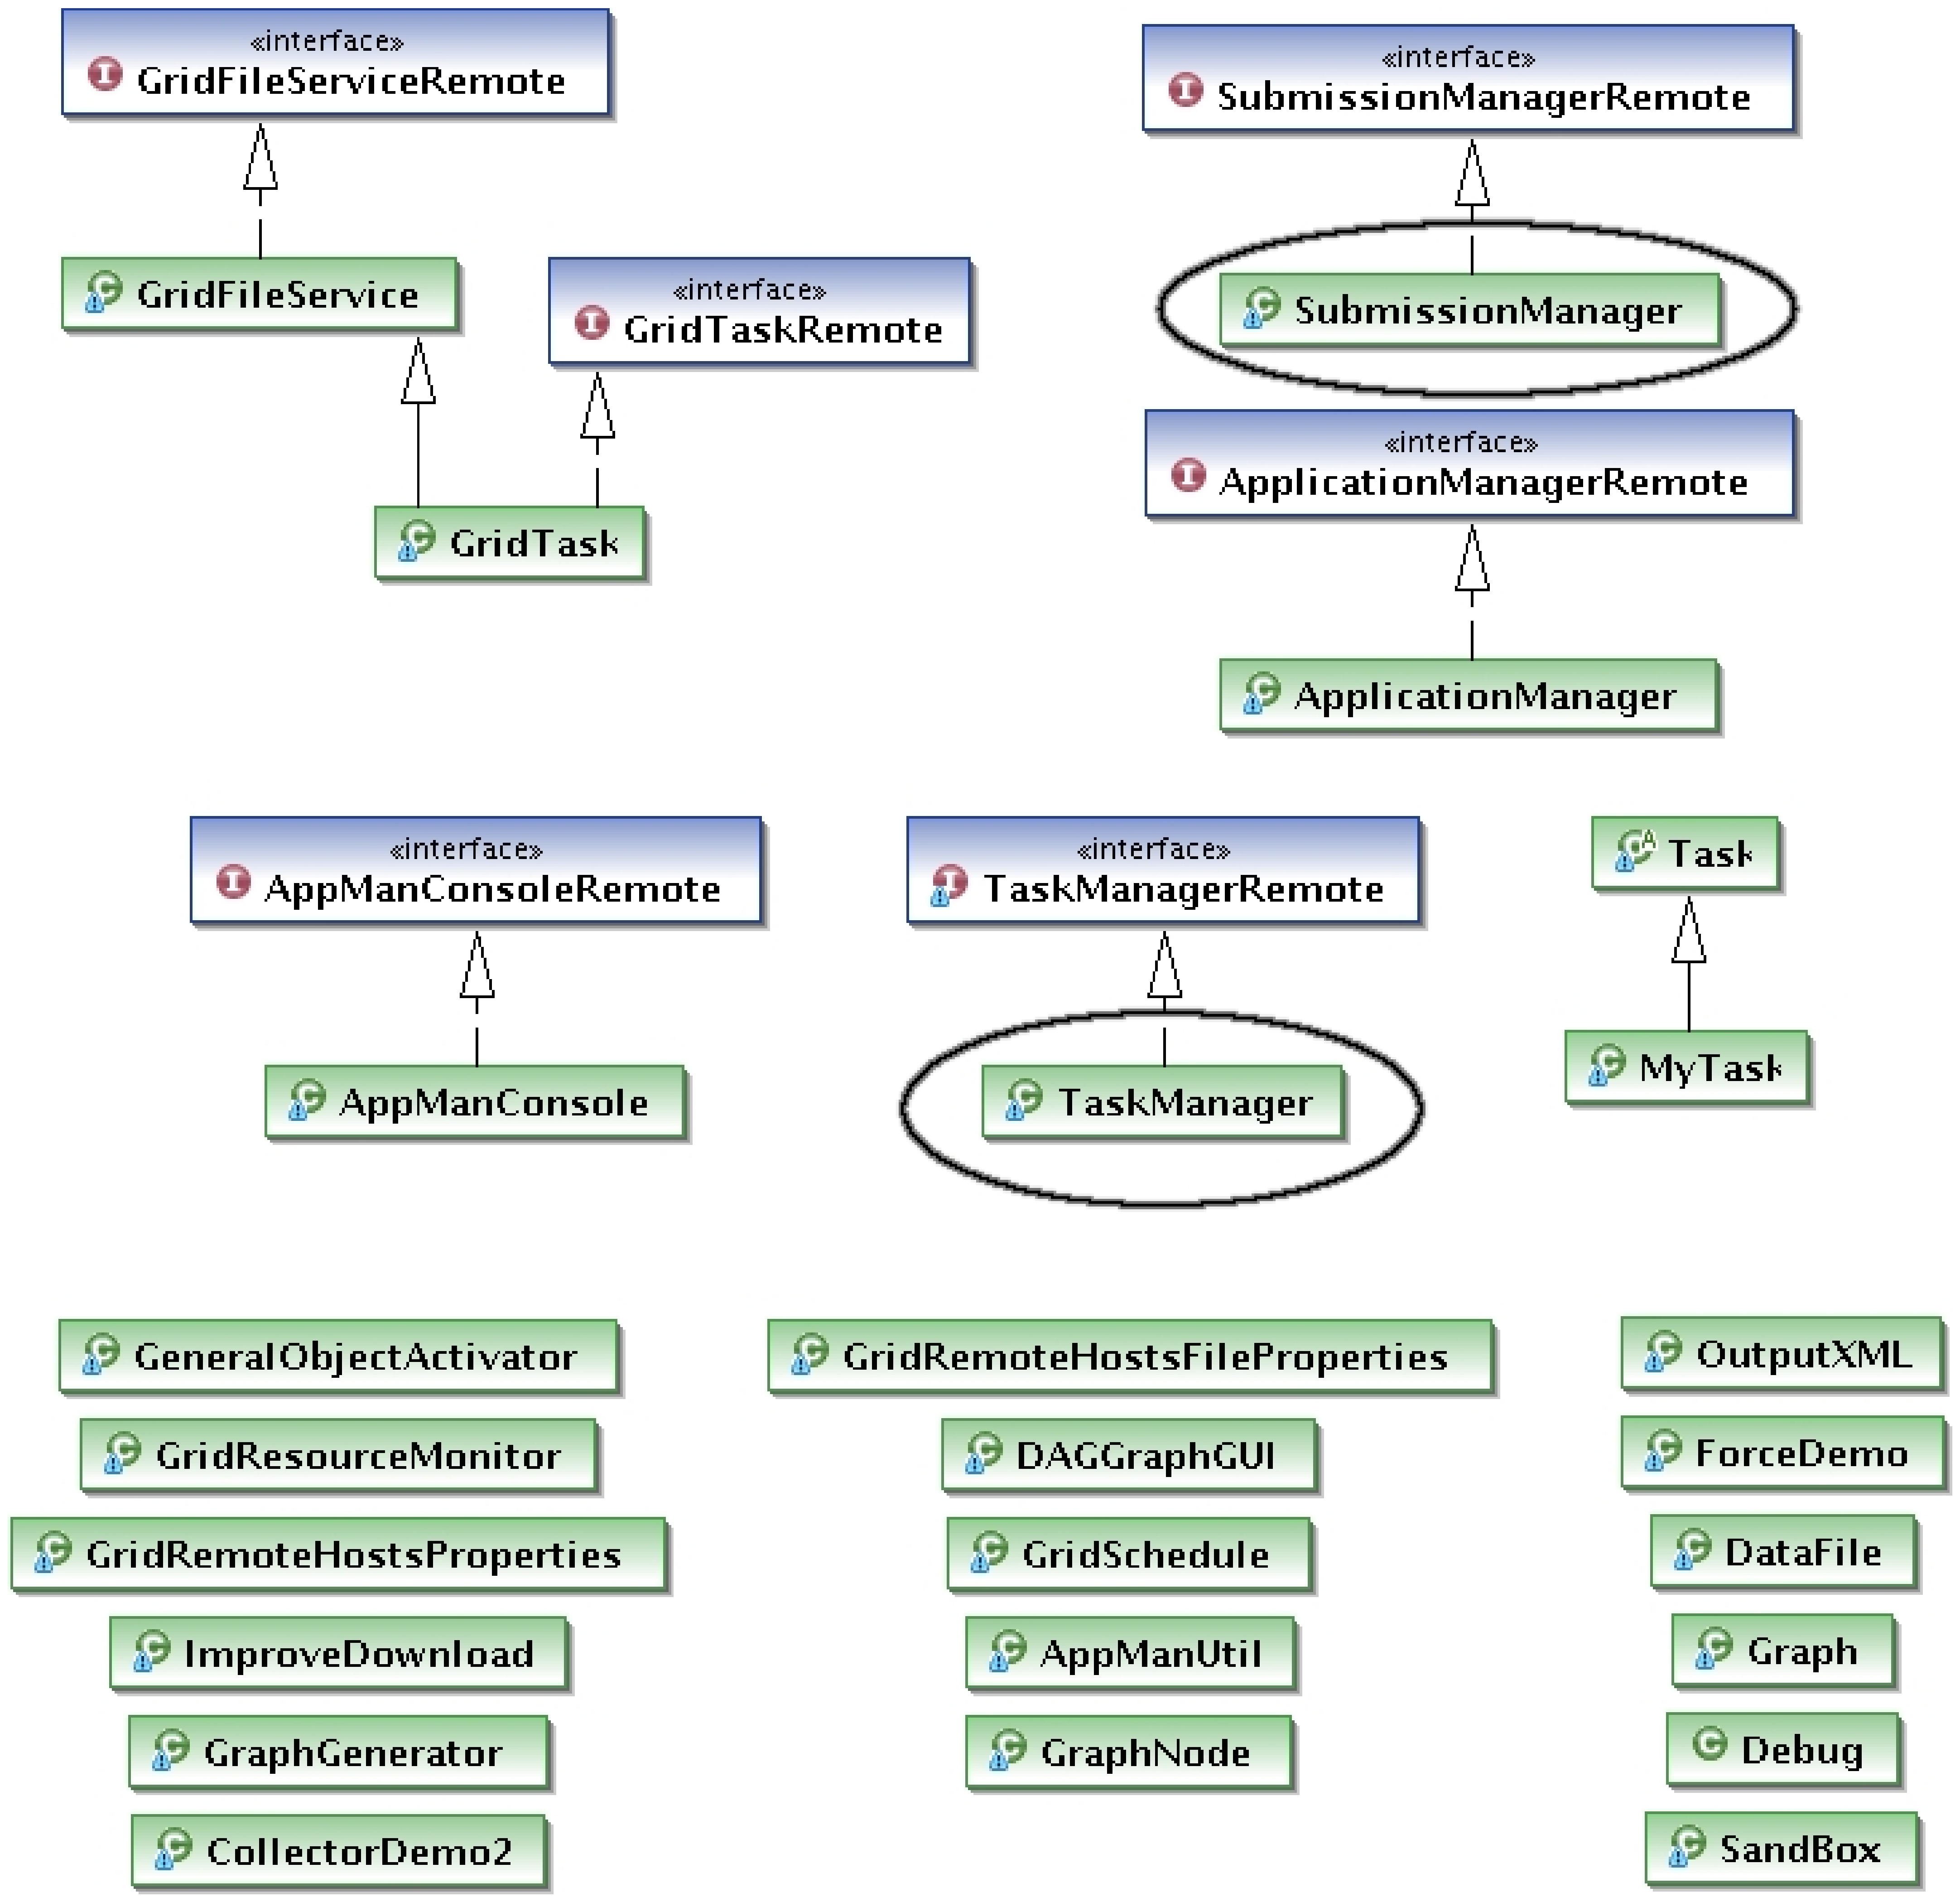
\includegraphics[scale=.16]{img/UML.eps}
\label{TaskManager}
\caption{Diagrama UML simplificado}
\end{figure}

Baseado no que foi analisado até o momento da confecção deste artigo, notou-se a necessidade de alteração na {\it Interface TaskManagerRemote} onde necessitará ser adicionado métodos que implementarão as especificações da DRMAA. Essa seria a melhor forma de implementação com a mínima interferência no código atual. Principalmente por existirem trabalhos nessa área \cite{Nobres2007}.

A presente proposta de pesquisa proporcionará uma maior dispersão geográfica para o AppMan pois, novos domínios adimistrativos (instituições) poderão fazer parte da grade em que se encontra. Contribuiria, também, para o AppMan ficar próximo de atingir o que propõem o modelo GRAND resolvendo o problema da necessidade do EXEHDA/AppMan estarem presentes em todos nós da grade. 

A Figura 4 demonstra como deverá ficar o funcionamento do AppMan após a realização do trabalho proposto. Os TMs nos nós locais contatam RMSs remotos despachando as tarefas para esses RMSs.

\begin{figure}[hpts]
\center
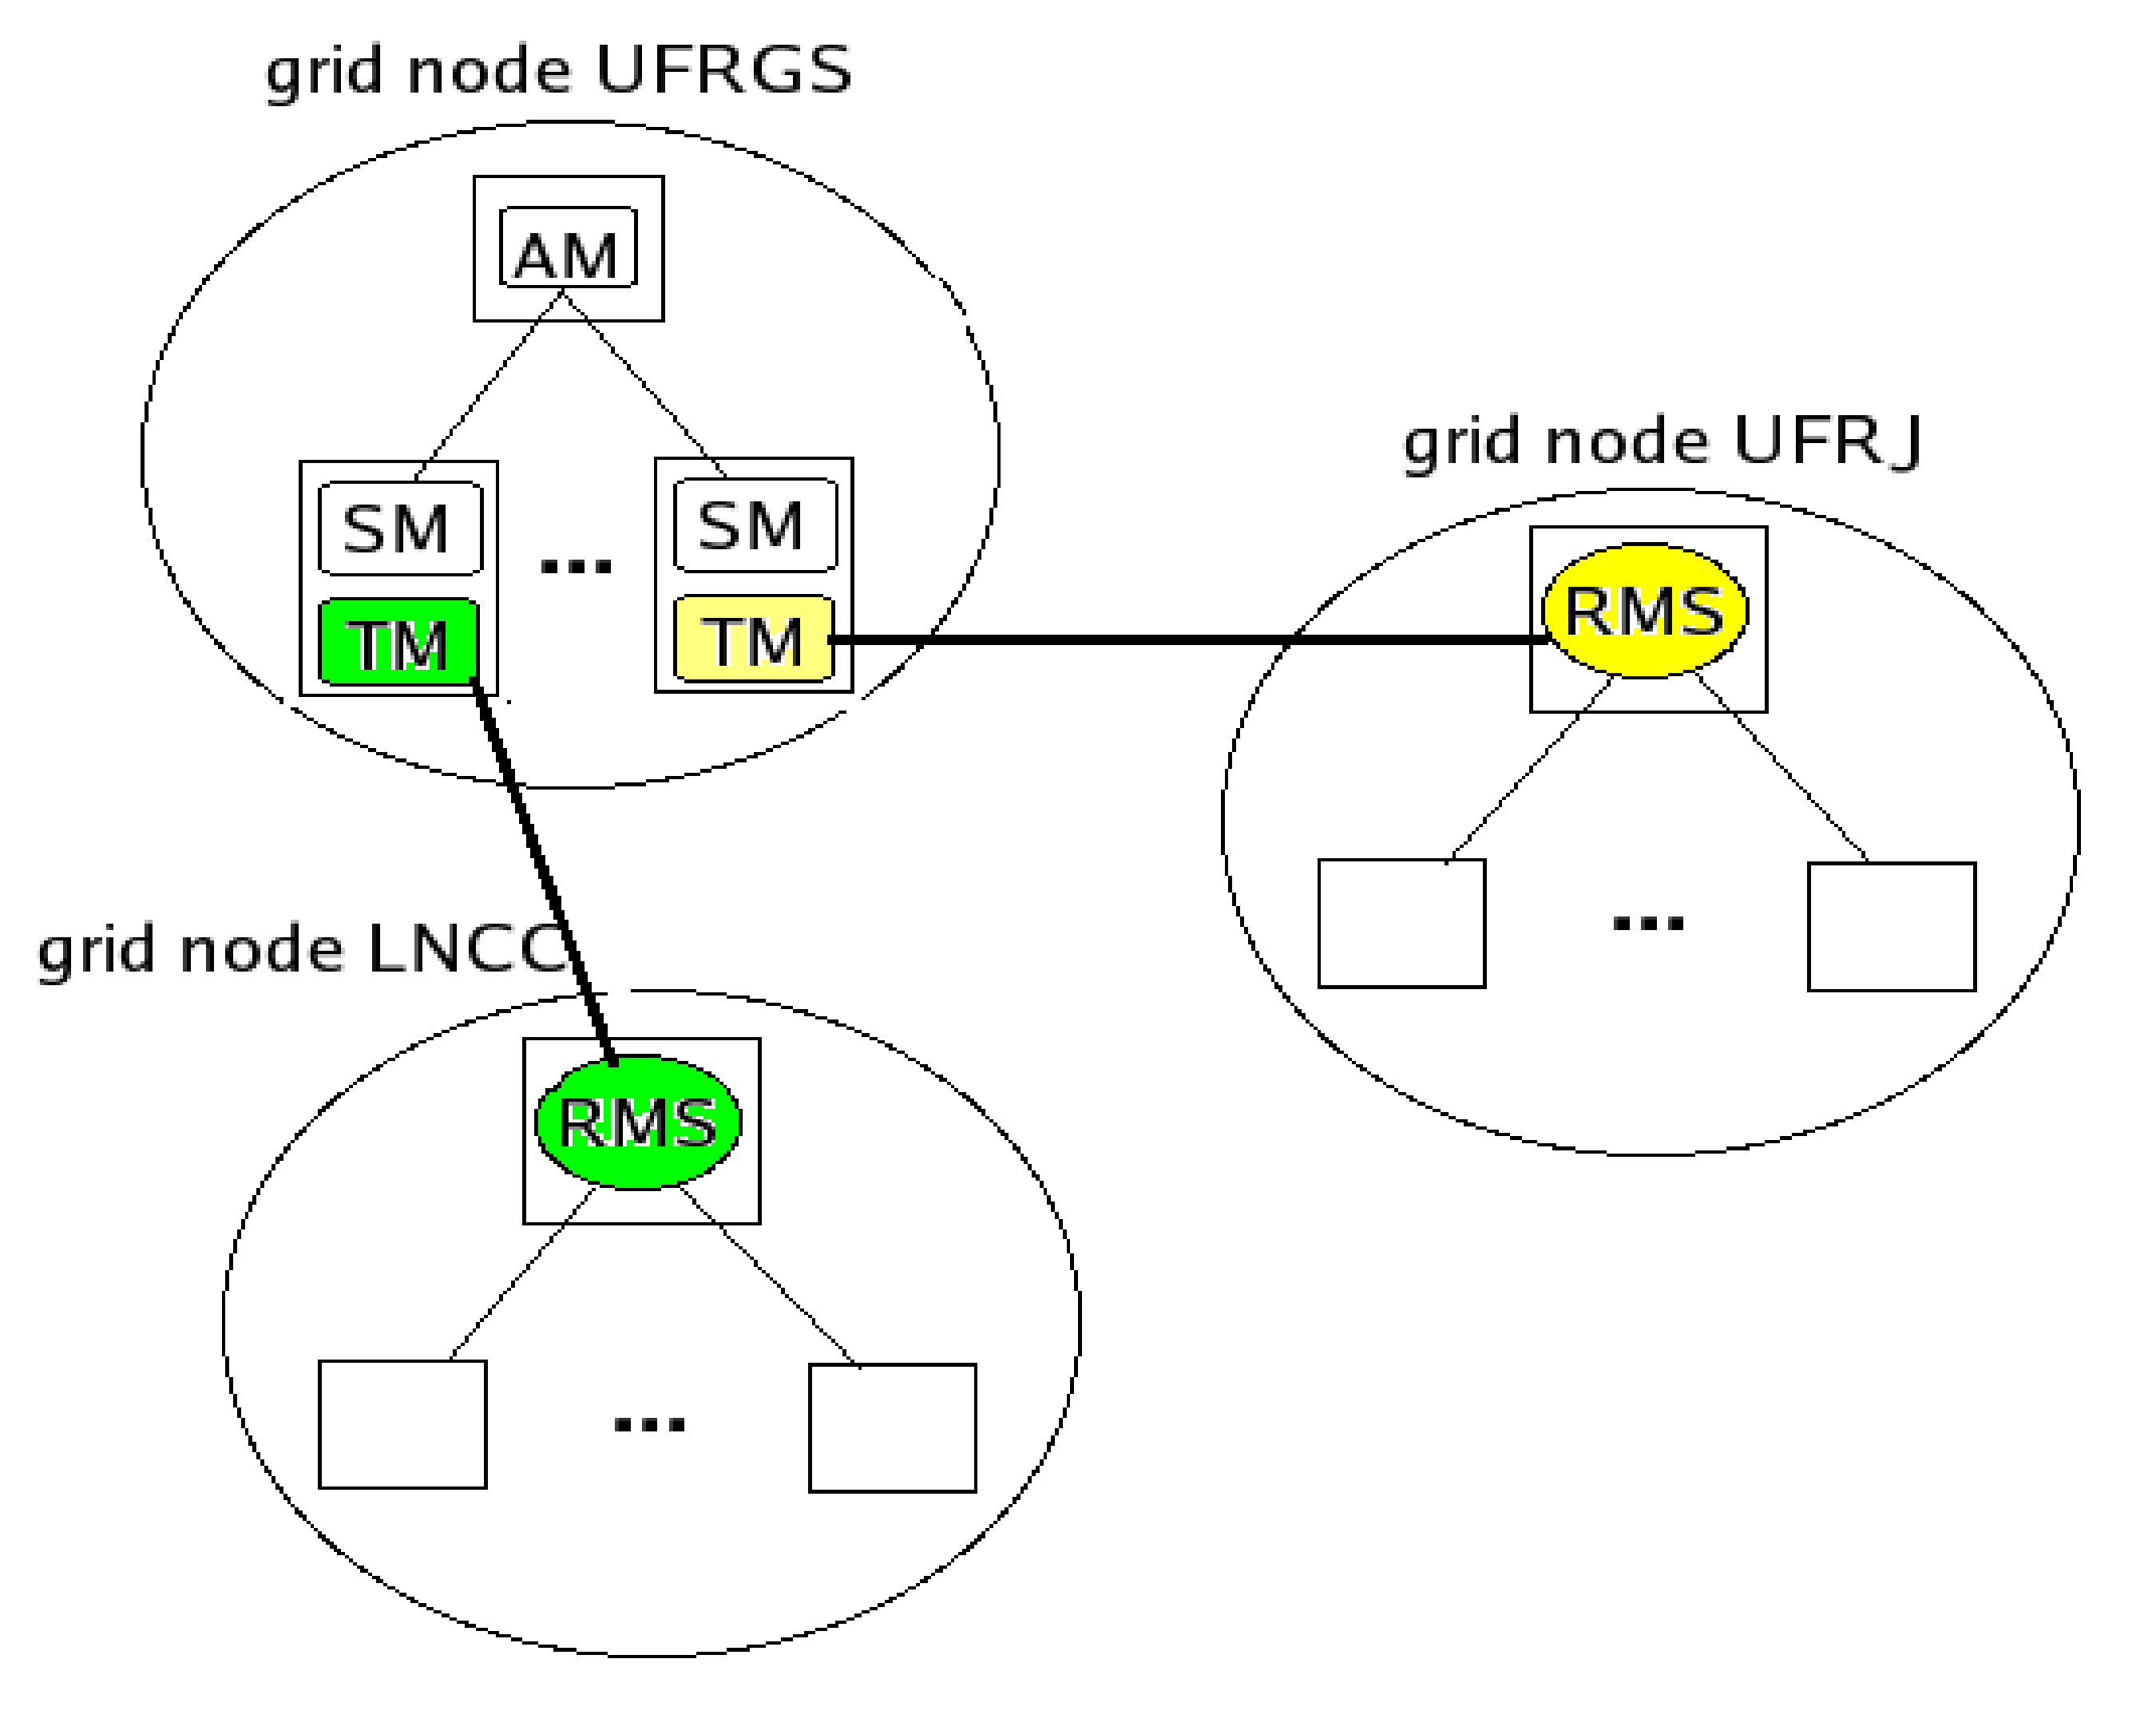
\includegraphics[scale=.2]{img/AppManRMS.eps}
\label{AppManRMS}
\caption{AppMan executando em um cenário com TMs comunicando com RMS}
\end{figure}

O modelo proposto para o TCC consiste em avaliar se a especificação DRMAA atende as necessidades do AppMan bem como realizar a integração do AppMan ao menos com um RMS.
		% Inclus�o do Capitulo de Modelo
	\chapter{Dados Experimentais}
\label{cap:Dados_Experimentais}

Este cap�tulo apresenta os resultados dos ...


Para a m�dia foi calculada a m�dia aritm�tica simples e para o desvio foi calculado atrav�s da f�rmula do desvio padr�o (n�o-polarizado ou n-1) escrita assim:

\begin{center}
\begin{math}
\sqrt{ \frac{n\sum x^{2} - (\sum x)^{2}}{n(n-1)}}
\end{math}
\end{center}



\section{\label{sec_Intrusao_Maquina}Intrus�o na M�quina}


A Tabela \ref{tab:intrusao_maquina} mostra o ...


\begin{table} [hbtp]
\begin{center}
\caption{Intrus�o nas M�quinas}
\label{tab:intrusao_maquina}
%\begin{footnotesize}
\begin{scriptsize}
\begin{tabular}{l|l|l|l|l|l}
	\hline
		{\bf Equipamento} & \multicolumn{3}{c|}{\bf Ocupa��o CPU} &  {\bf Mem�ria} &  {\bf Tam. Arq. Gerado}\\
				  &	M�x	&  M�d	& 	Desvio	  & 	  	   & 			    \\
	\hline
		Equip 1		  &  50 \%	& 24 \%	 & 	19 \%	  &   3 MB	   & 	17 Kbytes	    \\ \hline
		Equip 10	  &  49	\%	& 23 \%	 & 	16 \%	  &   5 MB	   & 	16 Kbytes	    \\ \hline \hline
		\bf{M�dia}	  &  49,7 \%	& 23,2 \%&	17,5 \%	  &  5,6 MB	   &	16,2 Kbytes	    \\ \hline
		\bf{Desvio Padr�o}&  0,48 \%	& 1,03 \%&	1,64 \%	  &  1,64 MB	   &	0,78 Kbytes	    \\ \hline



\end{tabular}
%\end{footnotesize}
\end{scriptsize}
\end{center}
\end{table}


	% Inclus�o do Capitulo de Dados Experimentais
	\chapter{Conclus�o}
\label{cap:Conclusao}

Neste trabalho apresentamos os principais aspectos que caracterizam ....

O modelo proporciona n�o s� informa��es de software ...

...

Finalmente, um trabalho futuro importante � ...

Todos os exemplos de refer�ncias: 

\begin{itemize}
 \item livro: \cite{jain91}
 \item cap�tulo de livro: \cite{fosterGridChapterBook98}
 \item artigo congresso: \cite{easygrid2005}
 \item artigo revista: \cite{condor2005}
 \item tese de doutorado: \cite{teseAdenauer}
 \item relat�rio t�cnico: \cite{kayserTRqualify2004}
 \item p�gina Web de projeto: \cite{GANGLIA2006}
 \item outros tipos de refer�ncia: \cite{pessoalRede}
 \item outro tipo de publica��o (online): \cite{globusToolkit}
 \item : \cite{}
\end{itemize}



		% Inclus�o do Cap�tulo de Conclus�o
	\appendix
\addcontentsline{toc}{chapter}{Ap�ndices}
\chapter {Documento XML do Sensor Completo}
\label{anexo:xml_completo}

\begin{scriptsize}
\begin {verbatim}
  <?xml version="1.0" encoding="utf-8" ?> 
 <Computador xmlns:BMS="http://n061/bms/link">
 ...
</Computador>

\end{verbatim}
\end{scriptsize}




%=============================
\chapter{GRID-ADL ABNF}
\label{appendix:gridADL}


%% listing - decrease fonte size%%
%\lstset{
%  basicstyle  = \scriptsize\ttfamily,
%}
%%
\begin{lstlisting}
;
; The input_file non-terminal is the starting point of this grammar
<input_file> = [ <graph_definition> ]
               [ <application_requirements> ]
               <set_of_task_definition>
               [ <transient_file_definition> ]
...
\end{lstlisting}

%% listing - return to previous value %%
%\lstset{
%  basicstyle  = \footnotesize\ttfamily,
%}
%%			% Inclus�o do Cap�tulo de Anexos
	%\bibliographystyle{abnt-alf}
\bibliographystyle{apalike}
\bibliography{biblio}
		% Inclus�o da bibliografia
\end{document} 
